\documentclass[border=4pt]{standalone}
\usepackage{amsmath,amssymb,amsfonts}
\usepackage{xcolor,colortbl,array,booktabs,multirow}
\usepackage{tikz}
\usepackage{pgfplots}
\pgfplotsset{compat=1.16}
\usetikzlibrary{arrows, automata, backgrounds, calendar, chains, decorations,
    matrix, mindmap, patterns, petri, positioning, shadows, shapes.geometric,
    trees, shapes, decorations.pathreplacing, calc, tikzmark, arrows.meta,
    intersections, fit, graphs, quotes, angles, decorations.markings}
\newcommand{\st}{\text{ s.t. }}
\newcommand{\x}{\mathbf{x}}
\renewcommand{\b}{\mathbf{b}}
\renewcommand{\c}{\mathbf{c}}
\newcommand{\A}{\mathbf{A}}
\newcommand{\y}{\mathbf{y}}
\newcommand{\z}{\mathbf{z}}
\newcommand{\R}{\mathbb{R}}
\newcommand{\RR}{\mathbb{R}}
\newcommand{\Z}{\mathbb{Z}}
\newcommand{\ZZ}{\mathbb{Z}}
\newcommand{\npcomplete}{NP-complete}
\providecommand{\true}{\text{TRUE}}
\providecommand{\false}{\text{FALSE}}
\tikzset{vertex/.style={circle,fill=black!25,minimum size=20pt,inner sep=0pt},
    edge/.style={draw,thick,-},weight/.style={font=\small},
    selected vertex/.style={vertex, fill=red!24},
    selected edge/.style={draw,line width=2pt,-,red!50},
    ignored edge/.style={draw,line width=2pt,-,black!20}}
\newcommand{\vect}{\vec}
\providecommand{\ds}{\displaystyle}
\providecommand{\longvect}{\overrightarrow}
\usepackage[normalem]{ulem}
\definecolor{ocre}{RGB}{243,102,25}
\providecommand{\leftB}{\left[}
\providecommand{\rightB}{\right]}
\tikzset{directed/.style={postaction={decorate,decoration={markings,mark=at position .65 with {\arrow{>}}}}},
    directed1/.style={postaction={decorate,decoration={markings,mark=at position .65 with {\arrow{>}}}}}}
\begin{document}
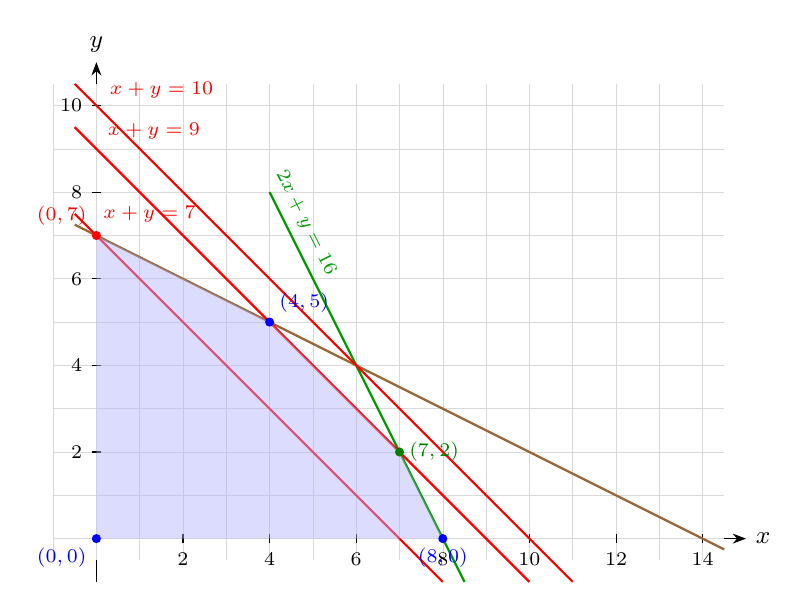
\begin{tikzpicture}[scale=0.55, >=Stealth,
    every node/.style={font=\small}]
  % Axes
  \draw[->] (-1,0) -- (15,0) node[right] {$x$};
  \draw[->] (0,-1) -- (0,11) node[above] {$y$};
  % Grid
  \draw[help lines, gray!30, very thin, step=1] (-1,-0.5) grid (14.5,10.5);
  % Tick labels
  \foreach \x in {2,4,6,8,10,12,14}
    \draw (\x,0.1) -- (\x,-0.1) node[below, font=\scriptsize] {\x};
  \foreach \y in {2,4,6,8,10}
    \draw (0.1,\y) -- (-0.1,\y) node[left, font=\scriptsize] {\y};

  % Constraint  2x + y = 16  (passes through (8,0) and (0,16))
  \draw[green!60!black, thick] (4,8) -- (8.5,-1) node[pos=0.1, sloped, above, font=\scriptsize] {$2x+y=16$};

  % Constraint  x + 2y = 14  (passes through (14,0) and (0,7))
  \draw[brown!80!black, thick] (-0.5,7.25) -- (14.5,-0.25);

  % Three values of b_1: x + y = 7, 9, 10
  \draw[red, thick] (-0.5,7.5) -- (8,-1) node[pos=0.05, above right, font=\scriptsize] {$x+y=7$};
  \draw[red, thick] (-0.5,9.5) -- (10,-1) node[pos=0.05, above right, font=\scriptsize] {$x+y=9$};
  \draw[red, thick] (-0.5,10.5) -- (11,-1) node[pos=0.05, above right, font=\scriptsize] {$x+y=10$};

  % Feasible region for b_1 = 9: vertices (0,0), (8,0), (7,2), (4,5), (0,7)
  \fill[blue!30, opacity=0.45]
        (0,0) -- (8,0) -- (7,2) -- (4,5) -- (0,7) -- cycle;

  % Vertex markers and labels
  \fill[blue] (0,0) circle (3pt) node[below left, font=\scriptsize, fill=none] {$(0,0)$};
  \fill[blue] (8,0) circle (3pt) node[below, font=\scriptsize, fill=none] {$(8,0)$};
  \fill[blue] (4,5) circle (3pt) node[above right, font=\scriptsize, fill=none] {$(4,5)$};
  \fill[red]  (0,7) circle (3pt) node[above left, font=\scriptsize, fill=none] {$(0,7)$};
  \fill[green!50!black] (7,2) circle (3pt) node[right, font=\scriptsize, fill=none] {$(7,2)$};
\end{tikzpicture}
\end{document}
